\documentclass[twocolumn]{article}
\usepackage[utf8]{inputenc}
\usepackage{amsmath} 
\usepackage{lipsum}
\usepackage{stfloats}
\usepackage{listings}
\usepackage{minted}
\usepackage{tcolorbox}
\usepackage[block=ragged]{biblatex}

\setminted[python]{breaklines, framesep=2mm, fontsize=\footnotesize, numbersep=5pt}

\usepackage{blindtext}
\usepackage[sc]{mathpazo}
\linespread{1.05} 
\usepackage{microtype} 
\usepackage{float}
\usepackage{graphicx}
\usepackage[english]{babel}
\usepackage[hmarginratio=1:1,top=32mm,columnsep=20pt]{geometry} 
\usepackage[hang, small,labelfont=bf,up,textfont=it,up]{caption}
\usepackage{booktabs} 
\usepackage{lettrine} 
\usepackage{enumitem}
\setlist[itemize]{noitemsep} 

\usepackage{abstract}
\renewcommand{\abstractnamefont}{\normalfont\bfseries} 
\renewcommand{\abstracttextfont}{\normalfont\small\itshape}

\usepackage{titlesec}
\renewcommand\thesection{\Roman{section}} 
\renewcommand\thesubsection{\roman{subsection}}
\titleformat{\section}[block]{\large\scshape\centering}{\thesection.}{1em}{}
\titleformat{\subsection}[block]{\large}{\thesubsection.}{1em}{}

\usepackage{fancyhdr} 
\pagestyle{fancy} 
\fancyhead{} 
\fancyfoot{} 
\fancyhead[C]{Financial Market Analytics $\bullet$ Data Science $\bullet$ July 2022} 
\fancyfoot[RO,LE]{\thepage} 
\usepackage{titling} 

\usepackage{hyperref} 

\setlength{\droptitle}{-4\baselineskip} 
\pretitle{\begin{center}\Huge\bfseries} 
\posttitle{\end{center}} 
\title{\textbf{Financial Market Analytics Project}} 
\author{%
\textsc{Cerabolini Aurora, Comensoli Paolo, Tritella Mirko}\\[1ex] 
\textsc{839327, 883147, 887196}\\[1ex] 
\normalsize University of Milano Bicocca \\ 
\normalsize MSc Data Science \\ %
\normalsize Academic Year 2021/2022 \\ 
}
\date{July, 2022} 
\renewcommand{\maketitlehookd}{%
\centering All codes, notebook, and the dataset folder can be viewed or downloaded here: \href{https://github.com/PaoloComensoli/MasterDegree/tree/main/FinancialMarketAnalytics}{GitHub Repository}
}

\begin{document}

% Print the title
\maketitle
\section{Introduction}

\lettrine[nindent=0em,lines=3]{I}\lowecase{n} this group project, we want to understand what are the structural characteristics that risk brings to real investment portfolios. For this reason, we need to build real portfolios that are focused on a specific level and type of risk. A portfolio is a collection of individual assets or securities and investors seek to diversify it instead of investing all of their wealth in a single or a few assets. With diversification, investors decrease the level of risk, in fact they want to maximize their return with less risk on their investment in a portfolio. To investigate the level of risk of individual stocks, we rely on the Single Index (beta) Model (SIM), proposed by William Sharpe in 1963, and then proceed to group the securities based on common characteristics in order to study them.
\subsection{Single Index Model}
Efficient portfolio construction with minimal risk for a given expected return can be achieved with the use of the Single Index Model proposed by Sharpe. The Single Index Model is based on the assumption that the fluctuations in the value of stock relative to other stocks do not depend on the characteristics of those securities alone. Relationships between securities occur only through their individual relationships with some indexes of business activity. Our index will be the Nasdaq-100. The equation of the Single Index Model links the returns of a single stock with the returns of the market index
\begin{equation}
r_i = \alpha_i + \beta_i(R_M) + \epsilon_i
\end{equation}
In this linear equation we have:
\begin{itemize}
    \item \texit{\(r_i\)} expected return on security \textit{i}
    \item \texit{\(R_M\)} is the return of the market
    \item \(\alpha\) is the intercept of the straight line or alpha coefficient: \(\alpha\) is often referred to as "excess return" and it measures the performance of an investment against a market index or benchmark that is believed to represent the movement of the market as a whole.
    \item \(\beta_i\) is the slope of the straight line or beta coefficient: beta is a measure of the volatility, or systematic risk, of a security or portfolio relative to the market as a whole. 
    \item \(\epsilon_i\) is the error term with the mean of zero and a standard deviation which is a constant
\end{itemize}
The variance of the security has two components namely systematic risk, or market risk, and unsystematic risk, or specific risk. The variance explained by the index is referred to as systematic risk and the unexplained variance is called residual variance or unsystematic risk.
\begin{equation}
Systematic Risk = \beta_i^2 \sigma_M^2
\end{equation}
\begin{equation}
\footnotesize{Unsystematic Risk = Total Variance - Sysmtematic Risk}
\end{equation}
\subsection{Benchmark Index}
The Nasdaq-100 (NDX) is one of the world's leading indices by capitalization. It includes 100 of the largest national (US) and international non-financial companies listed on the Nasdaq stock market by market capitalization. Within this index we find some of the major technology companies such as Apple, Amazon, Aphabet (Google), Facebook and Microsoft. The Nasdaq-100 undergoes quarterly reviews that occur in March, June, September and December and become effective with the closing values on the third Friday of the month. To become part of this index, stocks must have a daily trading volume of at least 200,000 pieces, have a total average market capitalization equal to or greater than 0.1\% of the average market capitalization of the Nasdaq-100 stocks and typically must have been listed for at least a couple of years - Figure [1].
\begin{figure*}[b]
\centering 
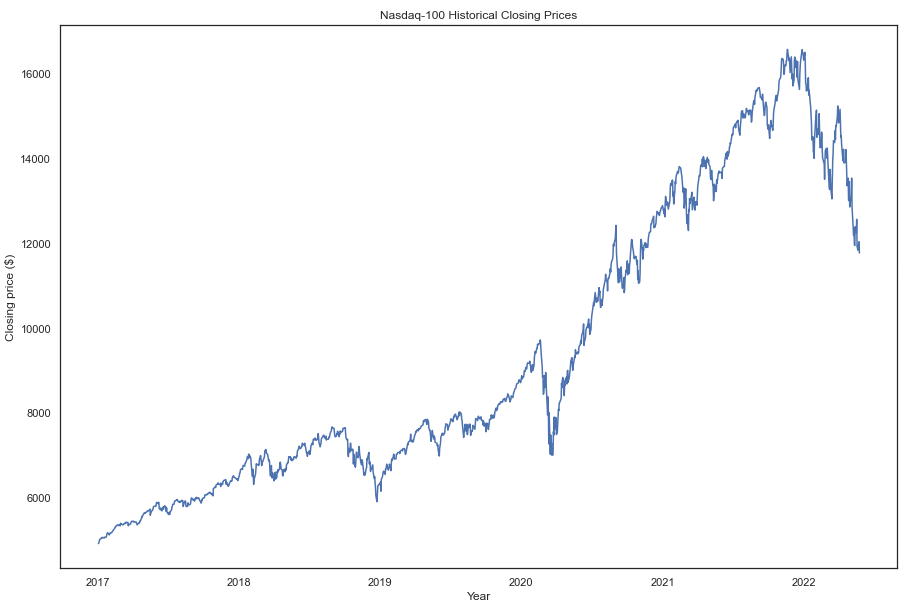
\includegraphics[scale=0.5]{ndx.png}
\caption{NASDA-100 Closing Prices}
\end{figure*}
\subsection{Dataset}
At this time (July 2022) there are 102 stocks within the Nasdaq-100. The complete list can be viewed here: \href{https://www.nasdaq.com/market-activity/quotes/nasdaq-ndx-index}{Nadaq-100}.
For the construction of the dataset, we downloaded the daily closing prices of these securities and of all those securities that were part of the index starting from 2017 (beginning of our historical series). We then managed the revisions of the securities by finding the incoming securities, the outgoing securities, and the effective date of exchange on the official Nasdaq website.
We used the Bloomberg terminal to download the data.\\
\rule{\linewidth}{0.4pt}
\vspace{-5 mm}
\begin{minted}{python}
closing_prices = pd.read_csv(CLOSING_PRICE_CSV)
closing_prices.head()

# Output in Figure [2]
\end{minted}
\vspace{-5 mm}
\rule{\linewidth}{0.4pt}



\begin{figure*}[t]
\centering 
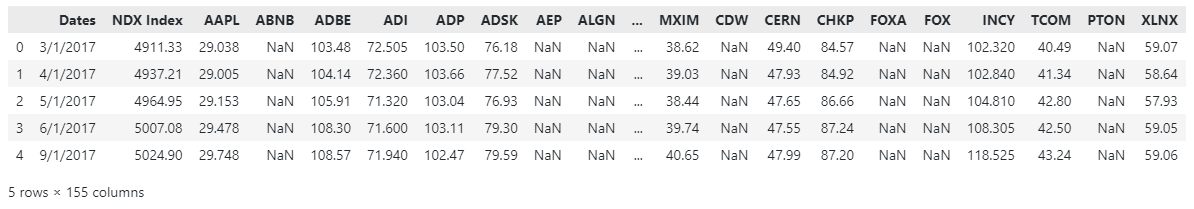
\includegraphics[scale=0.5]{closing prices.png}
\caption{Closing Prices}
\end{figure*}
When building the dataset we put attention to the survivorship bias. The survivorship bias indicates the tendency to consider only existing or "survivors" or "winners" stocks when measuring the performance of a portfolio. This is a bias linked to the "sample selection" in which observations that have already ceased to exist are not considered. For this reason, a portfolio's return may be overestimated, leading to overly optimistic conclusions. To avoid survivorship bias, we need to make sure that all data is present and that no longer present observations have not been omitted. To create a dataset that takes into account the revisions that took place during the analysis period, we also downloaded the historical series of daily prices even for those stocks that are no longer part of the index, but that are still within the U.S. stock market. By checking the date on which a certain change took place, indicated by \textbf{X}, between a security \textbf{A} (incoming) and \textbf{B} (outgoing), we set to \#N/A all the cells of B starting from X, valued the cells of A starting from X and setting to \#N/A all cells of A prior to X. In these 5 years that we are analyzing, it can happen that a stock was removed from the Nasdaq-100. We also had to look up the prices of those stocks that are no longer listed. In this case we had to consider the sale price or what was obtained from a merge.
\subsection{Risk-free rate}
In order to have somewhat more precise metrics, we decided to also consider the risk-free rate. The risk-free rate of return is the theoretical rate of return of an investment with zero risk. Since we are in the U.S. market we will use the U.S. 3-Month T-Bill as the risk-free rate. This is a useful proxy because the market considers there to be virtually no chance of the U.S. government defaulting on its obligations. For the data we actually used the Coupon Equivalent\footnote{\url{https://home.treasury.gov/policy-issues/financing-the-government/interest-rate-statistics}}. The Coupon Equivalent, also called the Bond Equivalent, or the Investment Yield, is the bill's yield based on the purchase price, discount, and a 365- or 366-day year.
\subsection{Pre-processing}
Starting from the closing prices of each title in our dataset and of our benchmark index, we calculate log returns. The log return can be calculated by simply taking a natural logarithm of the current price minus the logarithm of closing price of the previous day. One of the advantages is that the logarithmic returns are symmetric, this implies that logarithmic returns of equal quantity but opposite signs will cancel each other out. This means that if an investment of \$100 has a simple return of 50\% followed by a simple return of −50\%, the result will be \$75, while an investment of \$100 that give a logarithmic return of 50\% followed by a logarithmic return of −50\% will come back to \$100.
We use logarithmic returns to perform our regression which will allow us to build our portfolios.
\rule{\linewidth}{0.4pt}
\vspace{-5 mm}
\begin{minted}{python}
log_returns = np.log(closing_prices) - np.log(closing_prices.shift(1))
\end{minted}
\rule{\linewidth}{0.4pt}
\begin{center}
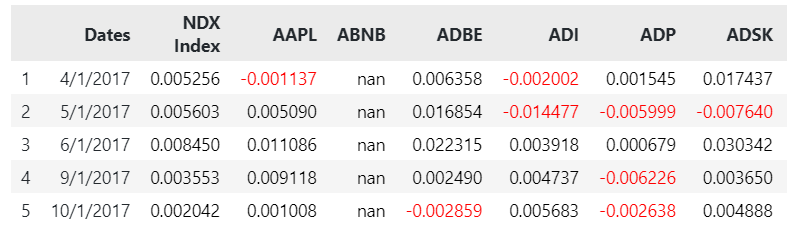
\includegraphics[scale=0.45]{logreturns.png}
\end{center}


\section{Building Portfolios}
\subsection{Ranking}
As we said previously with the Single-Index Model we can do a simple linear regression and the return of a stock \textit{i} is expressed by:
\begin{equation}
r_i = \alpha_i + \beta_i(R_M) + \epsilon_i
\end{equation}
By breaking down all the returns of the stocks under consideration into these components, and by using their properties, we can construct different rankings based on them or combinations of them. Through these rankings we can build our portfolios. To keep our tilted portfolios up to date, we will need to reevaluate these rankings weekly. In our study we will also try to see how these components can explain the returns of our portfolios. 
The following are the selectors used to build the portfolios:
\begin{itemize}
	\item{\textbf{Highest level of \(R^2\)}. R-squared measures how closely each change in the price of an asset is correlated to a benchmark}
	\item{\textbf{Lowest level of \(R^2\) and then high level of \(\sigma_i^2\) (total risk)}}
    \item{\textbf{Most aggressive stocks (high \(\beta_i\)) and most defensive stocks (low \(\beta_i\))}. Beta measures how large assets prices changes are in relation to a benchmark
    \item{\textbf{Stock with positive \(\alpha_i\) and eventually significant}}
    \item{\textbf{Stock with positive \(\alpha_i\) and also high \(\beta_i\)}}
    \item{\textbf{Highest and lowest level of \(\beta_i^2 \sigma_M^2\) (systematic risk)}}
    \item{\textbf{Stock with the highest absolute return \(r_i\)}, where absolute return is the return that an asset achieves over a specific period (in our case 180 days)}
    \item{\textbf{Excess returns over total returns, \(\dfrac{\alpha_i}{r_i}\) }
\end{itemize}
The selection of securities that are part of our portfolios is done by ranking. At the beginning of our procedure we calculate the first ranking on the previous 180 days. Rankings are obtained by going to sort the data according to specific selectors, such as highest r-square values or best absolute returns. We then calculate the current week's returns and re-run the previous procedure on the past 180 days by moving the window from week to week. We continue in this way until we get to the end of our data. To avoid look ahead bias, the stocks selected by the ranking procedure are based solely on past data relative to the week in which we will need to calculate returns. Even if a stock in that week were to drop out of the index or have completely different performance than in the past this does not matter. Within each ranking procedure what we do are the following steps:
\begin{enumerate}
\item We load the 180-day window of stock returns, and only the stocks that are present for all 180 days
\item For each security we perform a linear regression against the index (also with data referring to the same dates)
\item From the model we extract the values of the various parameters
\item Based on the selected selector, the best 10 titles will be chosen 
\end{enumerate}
Having obtained the list of securities we will then move on to the calculation of portfolio returns. For example to get the r-squared value:
\rule{\linewidth}{0.4pt}
\vspace{-5 mm}
\begin{minted}{python}
model = sm.OLS(title_returns, ndx_returns)
result = model.fit()

r2 = result.rsquared
\end{minted}
\vspace{-3 mm}
\rule{\linewidth}{0.4pt}
Regarding linear regression in our study, we used statsmodels\footnote{\url{https://www.statsmodels.org/stable/index.html}}. In addition to the list of titles, the ranking procedure also returns the table containing the values of all parameters. For this reason let's now go into a little more detail and look at the values that are returned by the model with regard to some selectors.\\\\
\textbf{Portfolio based on stocks with the highest level of R-squared}\\
We look at the first iteration of the selector with highest level of \(R^2\). The higher the R-squared number, the more correlated the asset is to its benchmark. A hypothetical portfolio with an R-squared of 0 has no correlation to its benchmark at all, while a portfolio with an R-squared of 1 matches the performance of its benchmark precisely. Looking at Figure [3]
\begin{figure*}[t]
\centering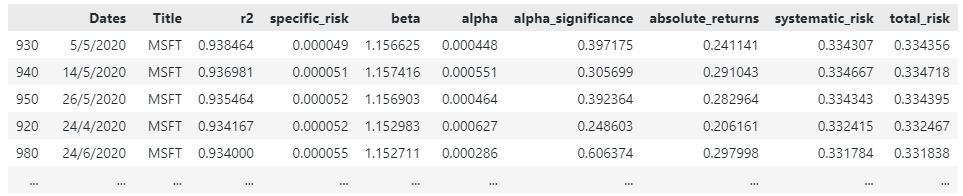
\includegraphics[scale=0.6]{microsoft.png}
\caption{R-squared selector first iteration result}
\end{figure*}
the first thing that jumps out is the fact that in this iteration, but which will remain true in subsequent iterations, is that within the portfolio we will find major American technology companies. This is actually not all that surprising, as they are giants from the standpoint of value and capitalization, and consequently it is plausible that they are the ones driving the economy and the underlying index. In this iteration we obtained stocks with r-square between 0.5 and 0.6. Good values but not outstanding.
\begin{figure*}[b]
\centering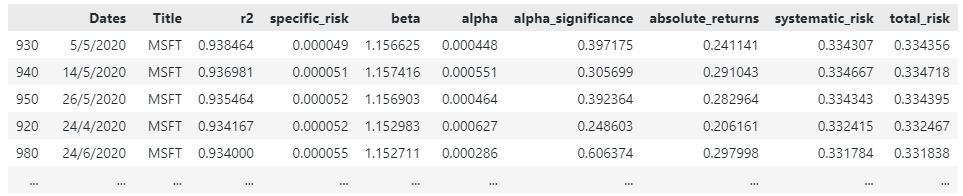
\includegraphics[scale=0.5]{microsoft.png}
\caption{Microsoft (NDX:MSFT) r-squared}
\end{figure*}
Over the whole series of this portfolio, the average R-square value is 0.68. In general, almost all stocks have a beta above one, and this means that they tend to be more aggressive than defensive stocks. The specific risk is very low and the alpha is also practically zero. The results proved to be as expected, and this portfolio performed slightly better than the index. As a final note the highest level of R-squared was obtained by Microsoft (MSFT) during 2020 with a maximum value of 0.93 - Figure [4].
\begin{figure*}[t]
\centering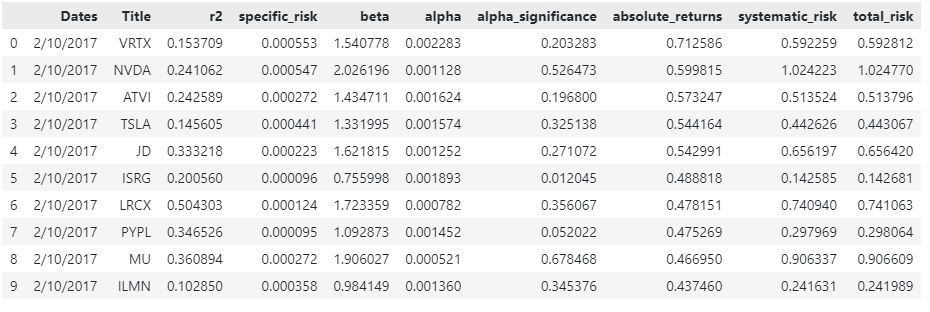
\includegraphics[scale=0.5]{absolute returns.png}
\caption{Absolute return selector first iteration result}
\end{figure*}
\\\\
\textbf{Portfolio based on stocks with best absolute return}\\
Look again at the first iteration of our procedure. Figure [5] shows the data of the first ten selected stocks. We can still see a high beta, a very small and nonsignificant alpha and a tendentially low r-square. What immediately jumps out at you, predictably, is the absolute return column. The first stock in the first six months of analysis achieved an absolute return of about 71\%. However, as we will see later, this portfolio did not perform exceptionally well, and underperformed the benchmark. The returns for the first week of this portfolio are:
\begin{center}
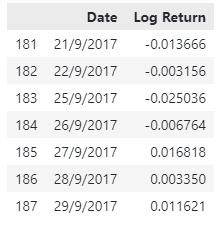
\includegraphics[scale=0.6]{absolutereturnfirstweek.png}
\end{center}
This is a good example of the fact that if a stock has performed well in the past, it does not necessarily perform well in the future. In fact, if we look at the returns of individual stocks in the first week we find that they were coming off a bearish period - Figure [6].
\begin{figure*}[t]
\centering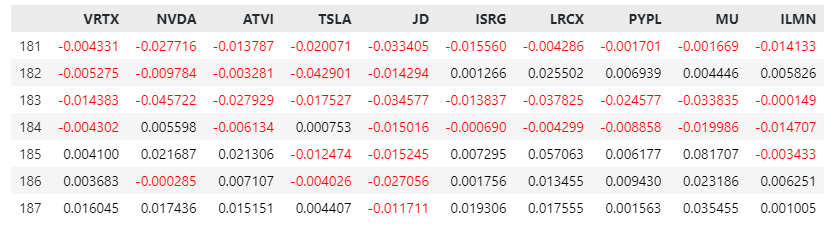
\includegraphics[scale=0.5]{bearishfirstweek.png}
\caption{First week of return (from day 181 to 187)}
\end{figure*}
\\\\
\textbf{Portfolio based on stock with positive alpha}\\
The excess return of a title relative to the return of a benchmark index is the title’s alpha. In other words it is the part of return of a stock due to firm-specific factors and therefore untied from macroeconomic events that affect the entire market. We know from theory that the CAPM specifies that alphas must be zero and that deviations from zero are the result of temporary disequilibria. In practice, however, assets may have non-zero alphas. For that reason alpha is also called “abnormal rate of return”, due to the fact that since markets are efficient, there is no way to systematically earn returns that exceed the broad market as a whole. Fund managers use both alpha and beta to evaluate an investment portfolio’s returns, in fact, positive value of alpha imply higher average excess return without the “cost” of any additional exposure to market risk. A value of 1.0 means that the title outperformed its benchmark index by 1\% and so the investment has a return in excess of the reward for the assumed risk. A negative number means that it has under-performed, or that it was too risky for the return, and if the alpha is zero, its returns match the benchmark, and so the return was adequate for the risk taken. As you can see from Figure [7], in our execution of the model we could not find stocks with a large alpha value.  The r-square value tended to be lower than in other portfolios.
\begin{figure*}[t]
\centering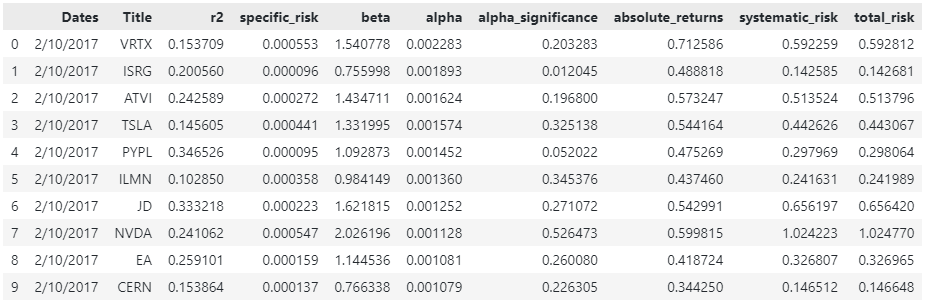
\includegraphics[scale=0.5]{positive_alpha.png}
\caption{Positive alpha selector first iteration result}
\end{figure*}
In this portfolio the average value of alpha is 0.0018. Adding the condition of selecting positive and significant alpha to the ranking procedure, however, returns an error because there are not 10 stocks with \texit{significant alpha} in each period. 
Going to look within the dataset of this portfolio we find that the range of beta values exceeds 2 in some cases, while in others it is negative (max negative -0.21) and with very low risks, both specific and systematic.
\begin{figure*}[t]
\centering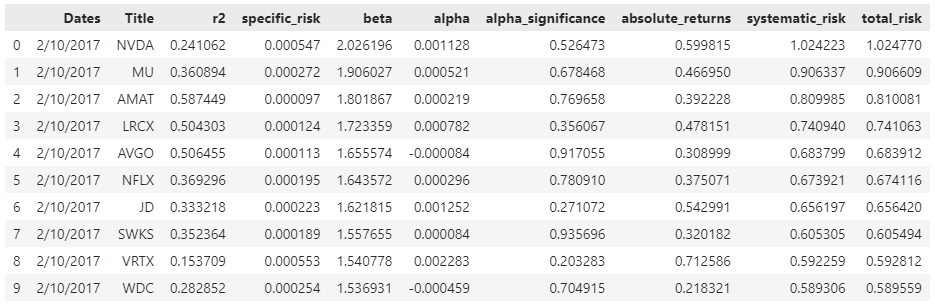
\includegraphics[scale=0.45]{highestSystematicRisk.png}
\caption{Highest systematic risk selector first iteration result}
\centering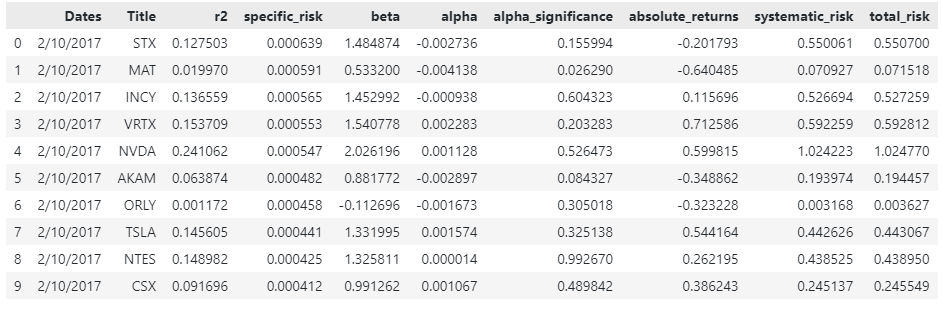
\includegraphics[scale=0.45]{highSpecificRIsk.png}
\caption{Highest idiosyncratic risk selector first iteration result}
\end{figure*}
\\\\
\textbf{Stocks with the highest systematic risk and highest Idiosyncratic Risk}\\
\texit{Systematic Risk} refers to the risk inherent to the entire market or market segment while \textit{Unsystematic Risk}, also known as specific risk or idiosyncratic risk, is the risk that is unique to a specific company or industry. Here we try to compare the results of the two portfolios containing the securities with higher systematic risk and higher specific risk - Figure [8] and Figure [9]. The specific risk values are not too high so it is not possible at first glance to see substantial differences. Despite this, the two portfolios performed quite differently. The portfolio with the highest level of systemic risk had an annualized return of 8.63\%, while the portfolio with the highest level of specific risk had a negative performance of -0.79\%. In terms of volatility, on the other hand, the difference is not so marked, the former 38\% while the latter 35\%, and thus less for the highest specific risk. In general, going by the data in the various iterations, ranking based on maximum specific risk often has negative absolute returns. However, the r-square and total risk are higher in the portfolio with higher systemic risk.
\\\\
\textbf{Stocks with the lowest total risk}\\
With this portfolio, we want to minimize the total risk of the components. The total risk is expressed as:
\begin{equation}
\small{Total Risk = Systematic Risk + Specific Risk}
\end{equation}
\begin{equation}
\sigma_i^2 = \beta_i^2 \sigma_M^2 + \sigma_{ei}^2
\end{equation}
If we continue looking at the first iteration, the results are as follows:
\begin{figure*}[t]
\centering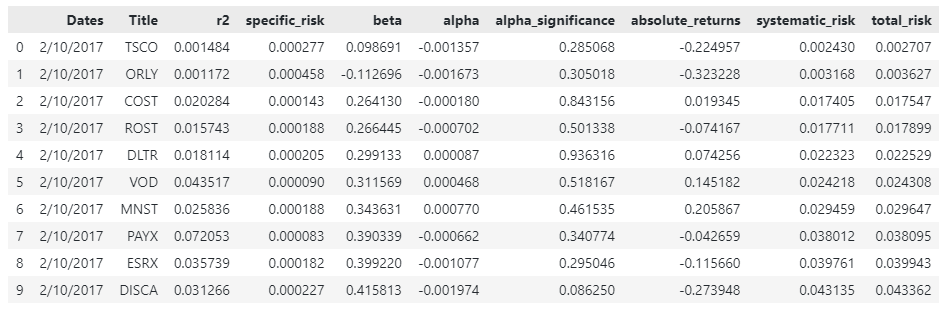
\includegraphics[scale=0.5]{minTotalRisk.png}
\caption{Minimum total risk selector first iteration result}
\end{figure*}
Total risk, as well as systematic and specific risk, of course, are very low. Interestingly, the values of r-square are very low and beta values are also very low, less than one. In fact, the stocks with the lowest risks are those that are defensive. Regarding alphas in this case we find several negative alphas, but still close to zero. Looking at the selected stocks, it is possible to see that the tech giants are not present, but instead there are retail companies, like TSCO (agriculture and garden products), ROST, mass media like Discovery (DISCA) or food and beverage companies like MNST.  
\subsection{How we calculate the portfolios returns}
At the end of each weekly iteration of the portfolio construction procedure we obtain a new list containing the ten titles based on some specific ranking. Before making the turnover of the assets inside our portfolios we need to calculate the portfolio return of the week just past. We look at the log returns dataset and we extract the seven rows of the week of the ten titles found within our portfolio. Since we decide to use a 1/N weight scheme we associate the same weight with each return of each individual stock. The daily return of the portfolio will be given by the sum of the returns of individual securities multiplied by their weight. In the first part of this report we talked about the \textit{survivorship bias} and so during the weekly calculation two exceptions may occur:
\begin{itemize}
    \item The stock was removed from the Nasdaq-100 but is still within the U.S. stock market
    \item The stock was removed both from the Nasdaq-100 and from the U.S. stock market, for example, because of an acquisition by another company
\end{itemize}
In the first case we have to go and get the closing price of the missing day (\texttt{closing\_prices\_removed\_titles} dataset), calculate the return and use that return for the particular day. The second case is more tricky. Based on our rankings, all the stocks that were part of the second exception were acquired or merged with another company and so we had to look up the price that the various shareholders received for each share. We searched for such information and loaded it into the dictionary \texttt{title\_out\_of\_the\_market}. In this case once the return is calculated, the title cannot be used on the remaining days for that week. This means that theoretically we need to decrease the number of stocks in the few remaining days and re-balance the weights within the portfolio, decreasing N by -1.
\subsection{Analyzing Returns and Volatility}
\begin{figure*}[t]
\centering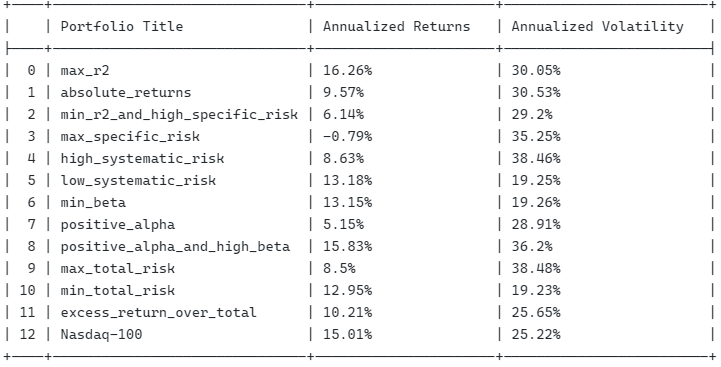
\includegraphics[scale=0.7]{baseMetrics.png}
\caption{Annualized return and volatility}
\end{figure*}
For each portfolio we calculated the annualized return and annualized volatility. For returns, we multiplied the average by 252, i.e. the average of trading days in a year of the NASDAQ and NYSE. On the other hand for the annualized volatility, we multiplied the standard deviation of returns by the square root of 252. Based on our data, starting from the beginning of 2017 to the first part of 2022, governed by strong uncertainty\footnote{\url{https://www.aa.com.tr/en/economy/nasdaq-sees-first-7-week-losing-streak-in-14-years/2594254}}, the annualized returns of the NDX is equal to 15.01\% with a volatility of 25.22\%. As we can see from Figure [11], the only two portfolios that did slightly better than the index are \texttt{max\_r2} and \texttt{positive\_alpha\_and\_high\_beta}. Both, however, have higher volatility. The portfolio related to titles with the highest specific risk not only under-performed the index but also achieved a negative return of -0.79\% with a great level of volatility. The portfolio with the greatest volatility, unsurprisingly, is the one\newpage that collects the securities exposed to the greatest total risk. A volatility of 38.48\% compared with a return of 8.5\%. In the opposite direction, the portfolio containing the securities with the lowest total risk obtains the lowest volatility over all. To get a clearer picture let us assume that we have invested \$1,000. We can then visualize the price chart:
\begin{center}
\vspace{0.5 cm}\hspace*{-7.8cm}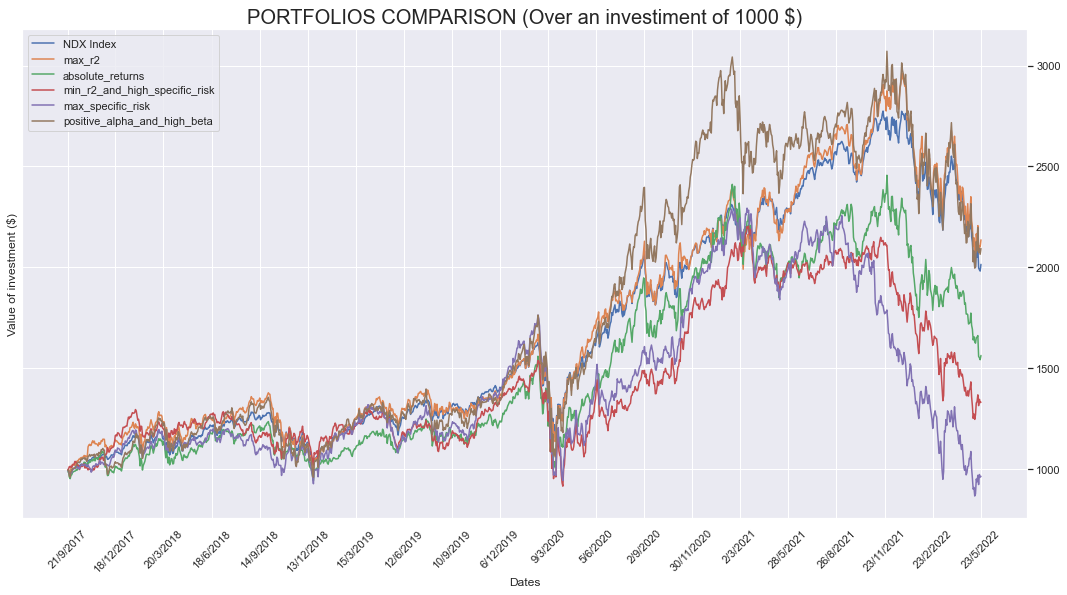
\includegraphics[scale=0.4]{portfoliosComparison.png} 
\caption{Different portfolios vs NDX}
\end{center}
\begin{center}
\centering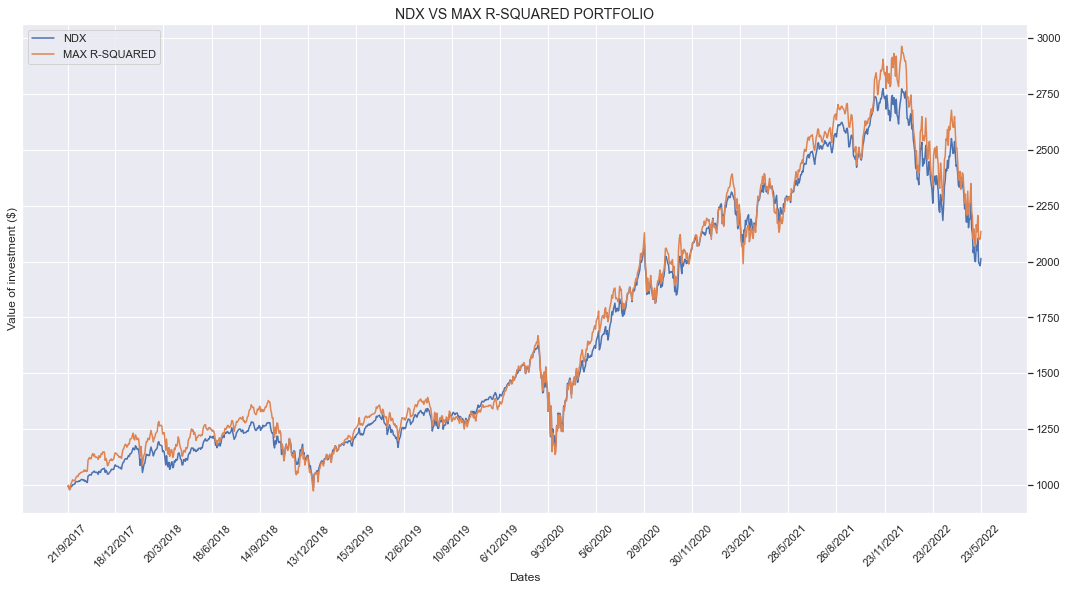
\includegraphics[scale=0.4]{ndxMarR2.png}
\caption{Highest r-squared portfolio vs NDX}
\end{center}
\begin{center}
\centering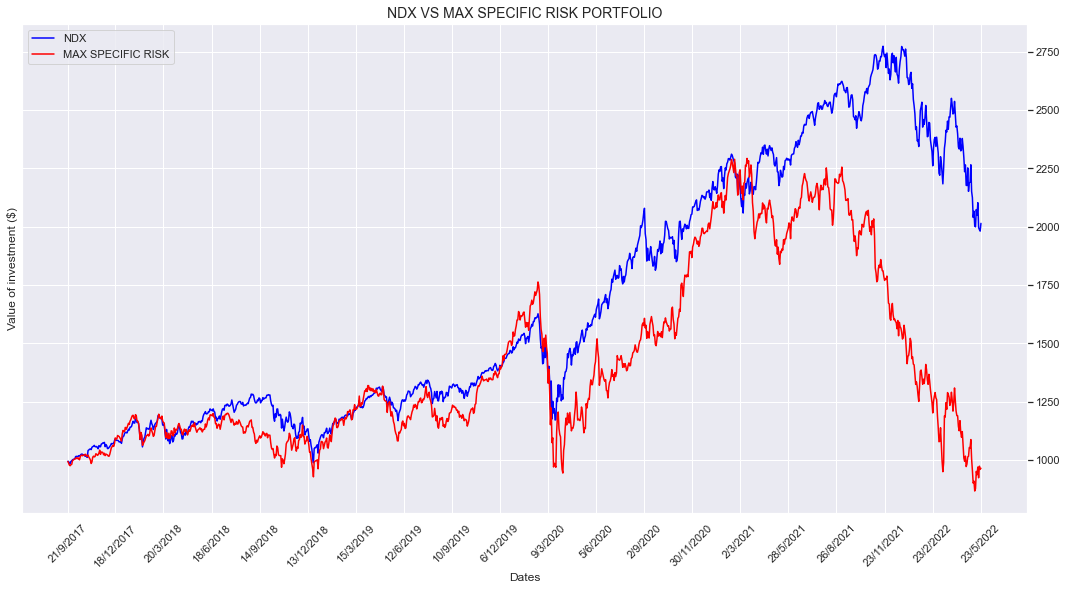
\includegraphics[scale=0.4]{ndxMasSpecificRisk.png}
\caption{Highest specific risk portfolio vs NDX}
\end{center}
\clearpage
\subsection{NDX vs Portfolio with Highest Specific Risk}
As we can see from the previous figure, this portfolio has been highly influenced by the events of the last period entailing a giant loss. Among the main causes we can find pandemic, inflation, energy and war. If we try to increase the number of securities within the portfolio, for example from 10 to 20 and then 30 what we see is a reduction in volatility, but still negative returns.
\begin{center}
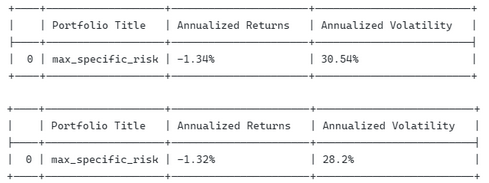
\includegraphics[scale=0.5]{asd1.png}
\end{center}
Of course, by reducing the number of securities, we also reduce diversification and thus achieve even worse performance.
\begin{center}
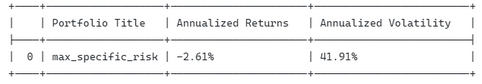
\includegraphics[scale=0.5]{asd2.png}
\end{center}
\section{Comparison with Metrics}
We calculate final statistics to compare the different tilted portfolios. The metrics we take into account are:
\begin{itemize}
    \item \textbf{Sharpe Ratio}: calculates an investment's average returns
    compared to its potential risks. It is calculated by subtracting the risk-free rate from the expected rate of return of the portfolio, and dividing the result by the standard deviation, otherwise known as the statistical measure of the asset's volatility. 
    The Sharpe ratio helps you determine whether the risk you've taken on has paid off in your returns, compared to the returns you might have seen without taking on risk. 
    A high Sharpe ratio means the risk is paying off in the form of above-average returns. However, a Sharpe ratio greater than zero is typically considered good. 
    In the formula, as a risk-free rate we used the US 3 month T bills: they are considered nearly free of default risk because they are fully backed by the U.S. government. On 14/07/2022, the sharpe ratio for nasdaq-100 was equal to -0.77. A negative Sharpe ratio means that the risk-free rate is higher than the portfolio's return. This value does not convey any meaningful information.
    \item \textbf{Maximum Drawdown}: expresses in percentage terms, and for a fixed period of time, the maximum loss of value that an investor can experience. In the history of an instrument or a portfolio, it is the distance between the absolute peak and the absolute minimum. A low maximum drawdown is preferred as this indicates that losses from investment were small. If an investment never lost a penny, the maximum drawdown would be zero. The worst possible maximum drawdown would be -100\%, meaning the investment is completely worthless.
    \item \textbf{Calmar Ratio}:  is a formula that measures the performance of an investment fund compared to its risk. It is a function of the expected annual rate of return and the maximum drawdown over the previous years. It is used to assess the success of various investment funds and make investment decisions. A high ratio suggests that the return of the investment was not at risk of significant drawdowns. On the other hand, a low ratio indicates that the risk of drawdown is greater.
    \item \textbf{Value at Risk}: it is a statistic that quantifies the extent of possible financial losses within a firm, portfolio, or position over a specific time frame. Risk managers use VaR to measure and control the level of risk exposure. One can apply VaR calculations to specific positions or whole portfolios or use them to measure firm-wide risk exposure. One measures VaR by assessing the amount of potential loss, the probability of occurrence for the amount of loss, and the timeframe.
    \item \textbf{Information Ratio}: provides the amount of excess return of the portfolio with respect to the reference benchmark for each unit of relative risk (represented by the tracking error) and allows to evaluate the manager's ability to outperform the benchmark in relation to the risk assumed (represented by the deviation from the benchmark). If the Information Ratio is positive, it means that the difference between profits and losses of these operations is positive, if the Information Ratio is negative, it means that the difference between profits and losses of the operations is negative.
    \item \textbf{Modigliani Ratio}: measures the returns of the portfolio, adjusted for the risk of the portfolio relative to that of some benchmark. To calculate the M2 ratio, we first calculate the Sharpe ratio and then multiply it by the annualized standard deviation of a chosen benchmark. We then add the risk-free rate to the derived value to give M2 ratio.
\end{itemize}
\subsection{The results}
\begin{figure*}[b]
\centering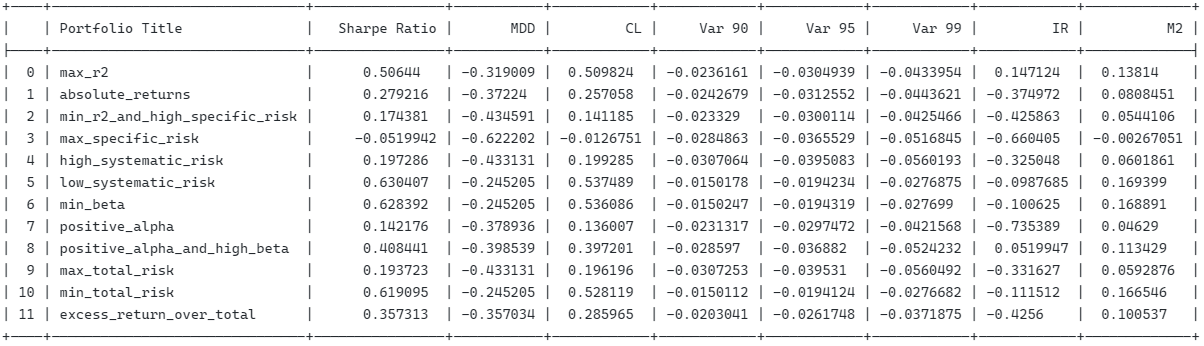
\includegraphics[scale=0.5]{advancedMetrics.png}
\caption{Advanced Metrics}
\end{figure*}
The table in Figure [12] shows the values of the previously described metrics, calculated for each portfolio. Looking at the Sharpe Ratio values, the portfolio that obtains the highest return per unit of risk is the one obtained by taking into consideration the 10 titles with the lowest Systematic Risk. This portfolio has a Sharpe Ratio value of 0.63, and is the highest value among the other portfolios. The other portfolios that have a high Sharpe Ratio value are the portfolio obtained considering the minimum values of the beta coefficient (SR = 0.628) and the portfolio obtained considering the lowest values of total risk (SR = 0.619).
Portfolio that has a Sharpe value close to zero (SR = 0.051, negative but really close to zero) is the one obtained considering the highest values of the specific risk: in these portfolios the investment's excess return is zero.\\
Considering the Maximum Drawdown values, the portfolio that has the maximum observed loss from a peak to a trough, before a new peak is attained, is the one built with the highest specific risk values. The MDD value of this portfolio is -0.622, this means that the maximum loss experienced by this portfolio was 62\%. The portfolios that have the lowest value of the MDD are those obtained with the minimum values of the beta coefficient, the minimum values of the systematic risk and the lowest values of total risk: all these three portfolios have a value of MDD equal to -0.245.\\
The highest Calmar ratio value is obtained from the portfolio built taking into account the minimum values of the systematic risk and the value is equal to 0.537. This value is considered good and this means that the portfolio is not at risk of significant drawdown.
The portfolio that is most at risk of drawdown is the one obtained with the positive alpha coefficient values: the Calmar Ratio value is 0.136.
The portfolio obtained with the highest values of specific risk has a negative Calmar ratio value but values below zero do not convey any meaningful information.
Observing the values of the Value at Risk calculated with a confidence level of 90\%, the portfolio that has the highest value of this metric compared to other portfolios is the one obtained with the highest values of the total risk: this portfolio has the risk of losing more than 3\% in only 10% of cases.
If we observe the values of the Value at Risk calculated with a confidence level of 95\% and with a confidence level of 99\%, we can see that the portfolio that has the risk of having a greater loss than the other portfolios is always the one obtained with the highest values of the total risk.\\
Looking at the values of the Information Ratio, only the portfolio obtained considering the highest values of R-squared and the portfolio with highest alpha and beta coefficients have obtained a positive value, and this means that investment management is active and efficient. In fact, the higher a value of the IR, the greater the manager's ability to achieve higher returns than the Benchmark Index. In this case, portfolio with highest values of R-squared has a higher IR value than portfolio with highest alpha and beta coefficients.\\
Considering the Modigliani Ratio, the portfolio that has the highest value (M2 = 0.169) is the one built considering the lowest values of the systematic risk. Compared to other portfolios, with the amount of risk taken, this portfolio is rewarding the investor more, in relation to the Benchmark Index and the risk-free rate of return.
\section{Non Compulsory Task}
\subsection{Momentum Strategy}
Momentum strategy is a system of buying stocks or other securities that have had high returns over the past months, and selling those that have had poor returns over the same period.
To implement this strategy, we consider the sample of 180 days (6 month momentum) and calculate the momentum of the stocks present in this window, we then select 1/3 of the stocks with the highest momentum value. After that, for each of the titles we perform the rolling regression and build the portfolios based on the previously described selectors, in the same way we did before without the momentum calculation. As we did previously, we re-balance the portfolio weekly and, each time we move the window forward seven-days, we calculate the momentum of the new stocks inside the window and take 1/3 of these stocks with the highest momentum value. After selecting the stocks with the highest momentum value, we identify a new stock ranking based on selectors. \\There are several ways to implement a momentum strategy. In our study we decide to implement the so-called Clenow Momentum\footnote{\url{https://www.amazon.it/Stocks-Move-Beating-Momentum-Strategies/dp/1511466146/}}. Clenow proposes an exponential regression in which we run a regression of log prices on time. However, in addition to the trend also the goodness-of-fit are important. In this way momentum is calculated by multiplying the annualized exponential regression slope of the past 180 days by the R-squared coefficient of the regression calculation:
\rule{\linewidth}{0.4pt}
\vspace{-5 mm}
\begin{minted}{python}
def get_clenow_momentum(title, days):
    prices = closing_prices[title].iloc[days: days + ROLLING_WINDOW_SIZE]
    prices_log = np.log(prices)
    x = np.arange(len(prices_log))
    slope, _, rvalue, _, _ = linregress(x, prices_log)
    m = ((1 + slope) ** 252) * (rvalue ** 2)
    return m
\end{minted}
\vspace{-3 mm}
\rule{\linewidth}{0.4pt}
After running the code, the result is as shown in the Figure [13] and [14].
\begin{figure*}[t]
\centering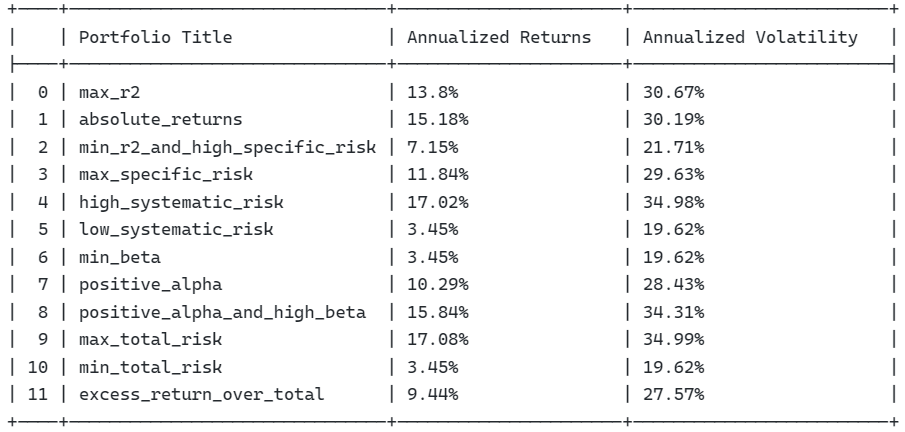
\includegraphics[scale=0.5]{momentumBase.png}
\caption{Annualized return and volality with Momentum}
\end{figure*}
\begin{figure*}[t]
\centering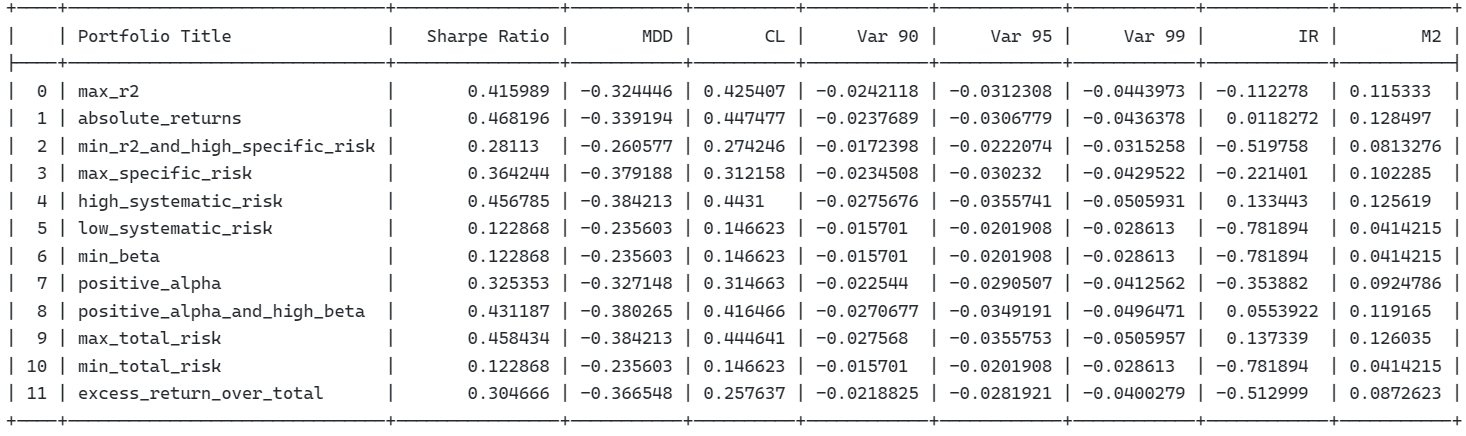
\includegraphics[scale=0.5]{momentumAdvance.png}
\caption{Advaced Metric with Momentum}
\end{figure*}
Depending on the type of selector, returns increased or decreased, more or less significantly. Variability, on the other hand, remained very similar. The most important change certainly concerns portfolios with the riskiest securities. The portfolio with the highest specific risk stocks went from negative to positive return, even better than others. And the portfolios with maximum total risk stocks and better absolute returns went from underperforming the index to overperforming it\footnote{The NDX annualized return was 15.01\% and annualized volatility of 25.22\%}. Looking at the Sharpe Ratio values, in this case the portfolio that obtains the highest return per unit of risk is the one obtained by taking into consideration the highest absolute returns. Portfolios that have the lowest Sharpe value are those obtained considering the lowest systematic risk, the lowest values of the beta coefficient and the lowest values of the total risk. Without the momentum calculation, the portfolio built with the lowest systematic risk was the one with the highest value of Sharpe Ratio. Considering the Maximum Drawdown values, the portfolios that have the maximum observed loss from a peak to a trough, before a new peak is attained, are those built with the highest systematic risk values and the highest total risk. The portfolios that have the lowest value of the MDD are the same obtained without the momentum calculation. The highest Calmar ratio value is obtained from the portfolio built taking into account the highest absolute returns. The portfolios that are most at risk of drawdown are those obtained with the lowest systematic risk, the lowest values of the beta coefficient and the lowest values of the total risk. Without the momentum calculation, the portfolio built with the lowest systematic risk was the one with the highest value of Calmar Ratio. Unlike before, no portfolio has a negative value of the Calmar Ratio. Observing the values of the Value at Risk calculated with a confidence level of 90\%, with a confidence level of 95\% and with a confidence level of 99\%, the portfolio that has the risk of having a greater loss than the other portfolios is always the one built with the highest values of the total risk and it is the same portfolio obtained without the momentum calculation. Looking at the values of the Information Ratio, there are four portfolios with positive values and the one with the highest value is the one obtained considering the highest values of total risk. 
\begin{figure*}[b]
\centering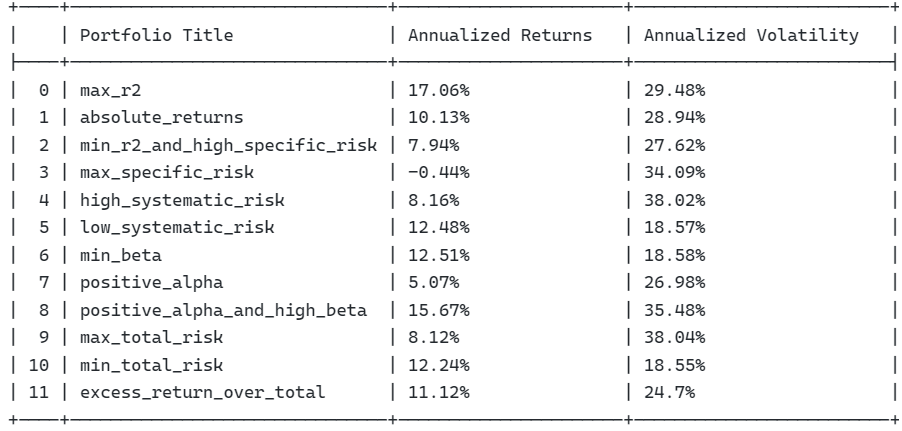
\includegraphics[scale=0.7]{newWeights.png}
\caption{Inverse Volatility Portfolios}
\end{figure*}
When we built the portfolios without the momentum calculation, the only portfolios with a positive value of IR were those built with highest alpha and beta coefficients and with highest R-squared. Here, the portfolio obtained with R-squared has a negative value. Considering the Modigliani Ratio, the portfolio that has the highest value is the one built considering the highest values of absolute returns, unlike when we built the portfolios without the momentum calculation where the portfolio with the highest value was the one with the lowest values of the systematic risk. Now, the portfolio built with the lowest values of the systematic risk is the one with the lowest value of M2.
\subsection{Inverse Volatility Weights}
In inverse volatility strategy the risk is measured with volatility, and assets are weighted in inverse proportion to their risk. An \textbf{inverse volatility weighted portfolio} is one in which highly volatile assets are assigned smaller weights and low volatile assets are allotted larger weights. The weights are given by,
\begin{equation}
W_i = \dfrac{\dfrac{1}{\sigma_i}}{\sum_j \dfrac{1}{\sigma_j}}
\end{equation}
In Figure [15] we can see the results. From these results we can see how depending on the type of portfolio the annual return either improved or slightly worsened. But the important thing you see is that in general volatility has decreased for everyone to a greater or lesser degree.
\subsection{Simple returns vs Log returns}
We have implemented a strategy where the return of our portfolios over any time period is the weighted sum of all the returns from each of the security. However we need to remember that log returns is a continuous compounded rate over time. When you add log returns, you compound. Across different stocks within the same time period, there are no compounding elements here, and so the sum of these returns represents only an approximation. So for computing portfolio return across contributions from securities within the same time period, simple returns might be a better choice. Let's look at an example:
\begin{center}
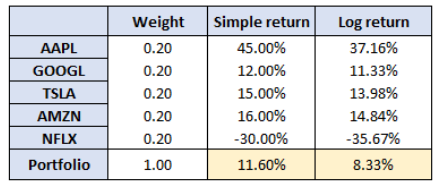
\includegraphics[scale=0.5]{logvsimple.png}
\end{center}
To analyze the results with simple returns, we converted the log returns to simple returns before calculating the daily portfolio return. The formula for conversion is as follows:
\begin{equation}
r = e^{ln(1+r) - 1}
\end{equation}
And in the end we got the results in Figure [16]
\begin{figure*}[t]
\centering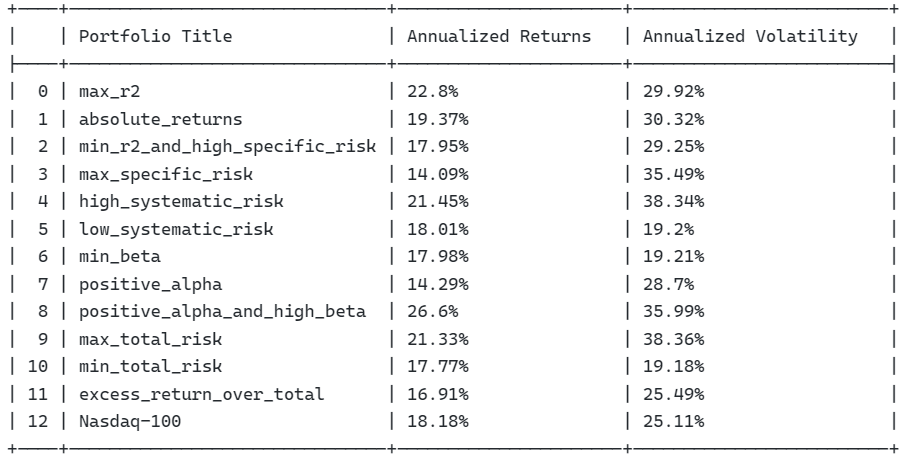
\includegraphics[scale=0.7]{simplereturns.png}
\caption{Simple Returns}
\end{figure*}



\begin{thebibliography}{99} 

\bibitem https://www.investopedia.com/ask/answers/102714/whats-difference-between-alpha-and-beta.asp
 

\bibitem https://www.borsaitaliana.it/notizie/sotto-la-lente/nasdaq.htm

\bibitem https://investmentcache.com/magic-of-log-returns-concept-part-1/

\bibitem https://chrischow.github.io/dataandstuff/2018-11-10-how-not-to-invest-clenow-momentum/

\bibitem https://www.quant-investing.com/blog/this-easy-to-use-adjusted-slope-momentum-strategy-performed-7-times-better-than-the-market

 
\end{thebibliography}



\end{document}
